\chapter{Private Data in PDFs}

In \chapref{ch:introduction} we recounted a case in which the UK
Parliament inadvertently posted a PDF on a website containing
sensitive information about nuclear subs. But this is hardly a lone
incident. PDFs have been responsible for many kinds of privacy leaks
since the format was introduced by Adobe in 1983

\section{The PDF Format}

Adobe created PDF in the 1990s as a format that would allow computer
users to view and print electronic documents. PDF was designed as a
single electronic container that could be distributed, viewed, and
printed on practically any modern computer system without the need to
install  software or fonts other than a general purpose PDF
reader. Adobe released programs for making and reading PDFs,
originally called Acrobat Distiller and Acrobat Reader, but it also
published the format specification and licensed the patents required
to implement it. Today there are numerous programs that can create,
display and even edit PDF files, and the format has been adopted as an
international standard (ISO 32000-1:2008)\cite{ISO32000-1:2008}.

% \subsection{Before PDF: PostScript}
% 
% Before PDF, electronic documents were typically distributed either as text
% files, such as the Internet RFCs, or as PostScript
% files. \emph{PostScript} is a programming language that Adobe Systems
% created in the 1980s. The key idea 
% of PostScript was that the language was interpreted by the printer, rather than 
% the computer. This allowed relatively small amounts of data to be sent to
% the printer, which would then render the page at the highest resolution
% the device supported. But it also meant that the computer would be
% freed from having to have drives for every different kind of printer
% that might ever be on the market.
% 
% Listing~\ref{hello.ps} below shows a simple PostScript program that draws a
% black box and the words ``Hello World!''  The output of the program
% (shrunk significantly) is shown at quarter size appears in
% \figref{hello-ps-figure}. 
% 
% \lstinputlisting[caption=A simple PostScript program,label=hello-ps-listing]{ch-pdf/hello-ps.ps}
% 
% Even without reading a PostScript manual you
% can draw some conclusions about the programming language simply by 
% inspecting the listing and the resulting output:
% 
% \begin{itemize}
% \item PostScript files begin with the magic number \verb|%!|.
% \item Strings are enclosed in parentheses. 
% \item Font names are preceded with slashes. (In fact, any literal name
%   can be put on the stack by preceding it with a slash.)
% \item Line drawing is performed with human-readable commands like
%   ``moveto'' and ``drawto''. 
% \item Arguments for commands come before the commands themselves,
%   implying that PostScript is a stack-oriented language.
% \item Because sometimes there are line breaks between commands and
%   other times there are not, you can reasonably infer that whitespace
%   is ignored in this file format.
% \end{itemize}
% 
% You can confirm these conclusions and learn more about PostScript by
% reviewing any one of the numerous online PostScript
% tutorial.\footnote{A particularly good online guide is \emph{A First
%     Guide to PostScript} by PJ
%   Weingartner. \url{http://www.tailrecursive.org/postscript/index.html}}
% You can also use a text editor (\S\ref{sec:text-editors}) to enter
% these characters into a file called \emph{hello.ps} and try opening
% the file with a PostScript viewer (\S\ref{sec:postscript-viewer}).
% 
% PostScript's initial use was inside the Apple LaserWriter, the first
% mass-market laser printer. There were inkjet printers, plotters, and
% large-scale laser printers before the LaserWriter, but each had their
% own language. With PostScript, application programs didn't have to
% separately understand how to generate print codes for each
% device. Instead, an application program could simply generate
% PostScript and know that the resulting page would be correctly
% printed. PostScript's most powerful features turned out to be the
% ability to distribute high-quality line art as encapsulated PostScript
% files that could embedded in other documents, scaled, transformed, and
% then printed---all with little work on the part of the application
% program. This, combined with the language's support for high quality
% typography, made PostScript one of the key enabling technologies of
% the 1980's boom in desktop publishing.
% 
% \begin{figure}
% 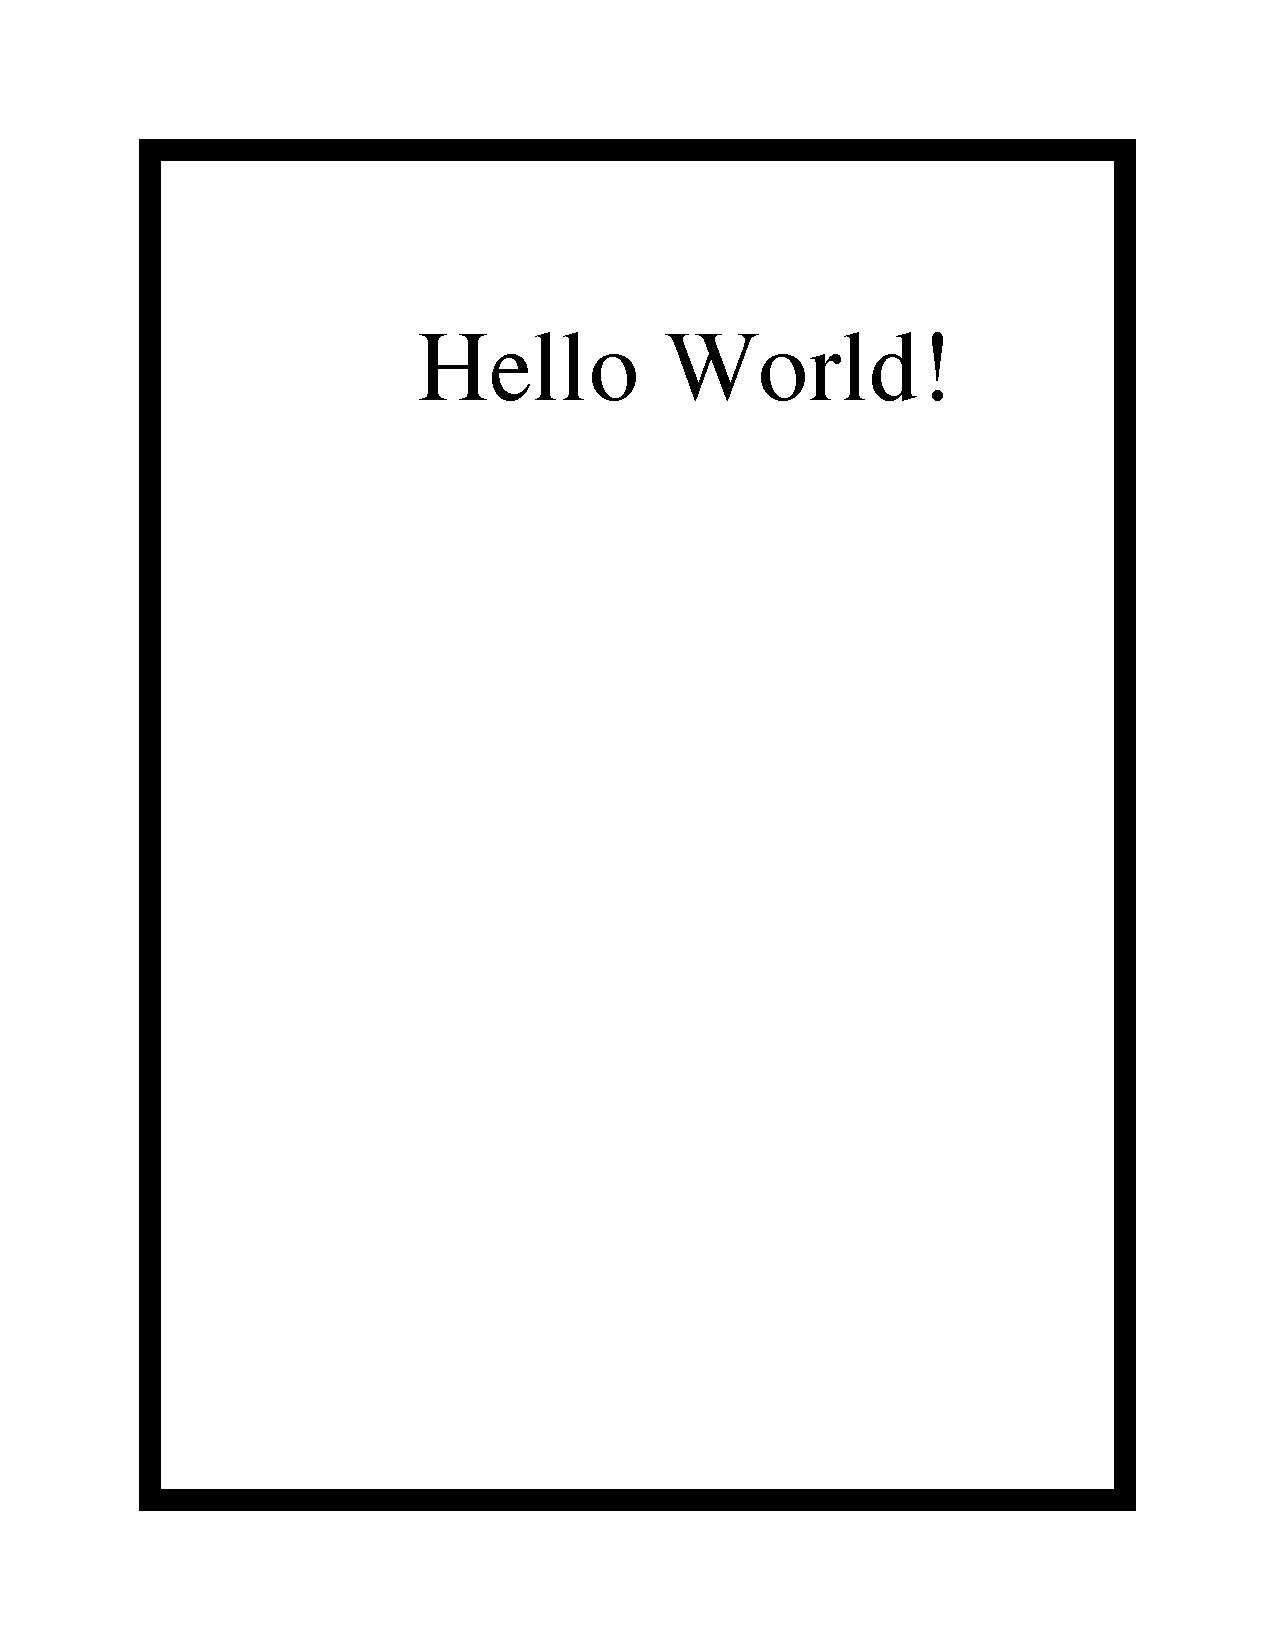
\includegraphics[scale=.25]{ch-pdf/hello-ps.pdf}
% \caption{The output of Listing~\ref{hello-ps-listing}, shrunk to 25\% of
%   the original size.}\label{hello-ps-figure}
% \end{figure}

\subsection{The PDF Specification}

PostScript's power made the language less than ideal as a universal
document format. First, the PostScript is somewhat verbose, so
PostScript files could get quite large. Second, the PostScript
execution context is not reset after each page, with the result that
PostScript viewers could not display pages out-of-order: in order to
show the contents of page 100, the viewer would first need to process
pages 1 through 99. Third, PostScript lacked support for many features
demanded in a modern electronic document format, such as data
encryption, digital rights management, and electronic forms.

The Portable Document Format (PDF) was introduced in 1993 to overcome
these problems with PostScript. Since then, PDF has become an
international standard for distributing born-digital documents, scans
of paper documents, and even electronic forms~ 
PDF was designed as, and as
such it includes direct support for typography, line art and digital
photographs, as well as for document elements such as pagination,
bookmarks and metadata. 

PDF is based on PostScript, but instead of being designed as a general
purpose programming language that produce printed pages, PDF is a
specialized file format. Like PostScript, PDF has
commands for drawing lines, embedding fonts and displaying text. But PDF also has direct support for
document structure; a variety of image and video compression
algorithms; electronic forms; digital rights management; and
cryptography. PDF supports embedded JavaScript for form validation
and other kinds of automation. Any page in a PDF document can be
rendered without reference to any other. 

Listing~\ref{hello-pdf-listing} presents a recast of
Listing~\ref{hello-ps-listing} as a PDF file. Below we summarize some
of the key differences:

\begin{itemize}
\item PDF files consist of a series of numbered objects. 
\item The \verb|moveto| command has been renamed \verb|m|, the
  \verb|lineto| command has been renamed \verb|l|, and so on.
\item At the end of the file a structure (called the cross-reference
  table) which has decimal offsets of the starting point of each object.
\item Finally, there is a trailer that provides information about the
  cross-reference table and the number of the first object required to
  render the document. 
\end{itemize}

Notice that the use of 10-digit decimal numbers means that PDF files
cannot be larger than 9,999,999,999 bytes in size. (Reportedly\footnote{\url{http://forums.adobe.com/thread/1041350}}, there
are additional limits in 32-bit PDF rendering applications.)





PDF gained significant popularity in part because it could be used to 
distribute documents without the  risks of embedded viruses and
privacy-leaking metadata, and because PDF files could not be readily
modified after they were produced and distributed. But as PDF's popularity grew, additional
features were added to both the standard and Adobe's PDF Acrobat
reader. Today PDF can hold arbitrary files as attachments, PDF can
contain JavaScript programs, and PDF can hold significant amounts of
metadata. PDF files can also be edited with a wide variety of
programs, including the open source InkScape program.


If you want to understand the internal PDF specification, you will have a much
easier time reading one of the earlier manuals than the later ones:

\begin{tabular}{lll}
Version & Year & Pages \\
\hline
PDF 1.2 & 1996 & 396 \\
PDF 1.3 (second edition) & 2000 & 696 \\
PDF 1.7 (part 1) & 2008 & 756\\
\end{tabular}



\section{Improperly redacted data}
\section{High-resolution JPEGs}
\section{High-resolution line drawing}
medical information leakage.
\section{Metadata}
\section{References}

\bibentry{nsa-pdfs}


